%\documentclass[10pt]{beamer}
\usepackage[utf8]{inputenc}
\usefonttheme{structurebold}
\usepackage{pgfpages}

%\usepackage{graphicx}
%\usepackage{amssymb}
%\renewcommand{\labelitemi}{$\bullet$}
%\usepackage[inline]{enumitem}
\usepackage{multirow}
%\usepackage{chngpage}
%\usepackage{pdflscape}
\usepackage{rotating}
\usepackage{longtable}
\usepackage{tabularx}
\usepackage{eurosym}

\usepackage{hyperref}
\usepackage{listings}

\usepackage{color}
\definecolor{gray}{rgb}{0.4,0.4,0.4}
\definecolor{darkblue}{rgb}{0.0,0.0,0.6}
\definecolor{cyan}{rgb}{0.0,0.6,0.6}

\lstset{
  tabsize=3,
  basicstyle=\ttfamily,
  columns=fullflexible,
  showstringspaces=false,
  commentstyle=\color{gray}\upshape 
}

\usepackage{caption}
\captionsetup{font=scriptsize,labelfont=scriptsize}
\setbeamertemplate{caption}[numbered]



\definecolor{istblue}{RGB}{0,157,224}
\definecolor{istgrey}{RGB}{70,85,95}
\definecolor{almostwhite}{RGB}{240,240,240}

\setbeamercolor{block title}{use=structure,fg=white,bg=istblue}
\setbeamercolor{block body}{parent=normal text,use=block title,bg=almostwhite}


\setbeamercolor{structure}{bg=white, fg=istblue}
\setbeamercolor{palette sidebar primary}{fg=istgrey}
\setbeamercolor{frametitle}{fg=istgrey}
\setbeamercolor{title}{fg=istblue}


\setbeamercolor{headfootlinecolor}{fg=black,bg=istblue}

\setbeamertemplate{footline}{%
  \begin{beamercolorbox}[sep=1em,wd=\paperwidth,leftskip=0.5cm,rightskip=0.5cm]{headfootlinecolor}{\textcolor{white}{} \hspace*{\fill} \textcolor{white}{Cloud-based Facility Management Benchmarking}}
   \end{beamercolorbox}%
}

\useoutertheme{sidebar}
\useinnertheme{circles}
\setbeamertemplate{itemize items}[circles]

\setbeamertemplate{blocks}[rounded][shadow=true]


\title[]{\usebeamercolor[bg]{white}Homophilic Self Organizing Feature Maps }
\author[]{\usebeamercolor[bg]{white}Bernardo Simões\\ \scriptsize Instituto Superior Técnico \\
}

\logo{
\includegraphics[scale=0,1]{images/istlogo}}


\AtBeginSection[]
{
\begin{frame}{Outline}
\tableofcontents[currentsection]
\end{frame}
\note[itemize]{
\item Current Section
}
}

\setbeamertemplate{frametitle continuation}{(\insertcontinuationcount)}

\begin{document}
\defbeamertemplate*{title page}{customized}[1][]
{
  \centering
  \usebeamerfont{title}\usebeamercolor[fg]{almostwhite}\inserttitle\par
  \usebeamerfont{subtitle}\usebeamercolor[fg]{almostwhite}\insertsubtitle\par 
  \bigskip
  \usebeamerfont{author}\insertauthor\par
  \bigskip
  \usebeamerfont{institute}\insertinstitute\par
  \usebeamerfont{date}\today\par
}


\begingroup
\setbeamercolor{background canvas}{bg=istblue}

\hspace{-40pt}
\begin{frame}[plain]
    \titlepage
    \vspace{-7cm}
    \begin{figure}
    \begin{center}
        
\includegraphics[scale=0.2]{images/istlogoazul}
    \end{center}
    \end{figure}
\end{frame}
\endgroup


\begin{frame}{Outline}
	\tableofcontents
\end{frame}
\note[itemize]{
  \item Explain the outline of the presentation
}


\section{Introduction}

%====================================================================================

%Vou começar por fazer uma introdução ao tema do Facilities management, passando por referir o problema que esta tese tenta resolver, Vou mostrar o que foi feito em termos de trabalho relacionado, nomeadamente standards, literatura cientifica e softwares existentes. Vou falar sobre a solução proposta e como a podemos validar. Por fim, vou falar das conclusões que podemos retirar.

\begin{frame}{Facilities Management}

	\begin{itemize}

	\item Rationalizes expenditures related to facilities \\

	\vspace{0.5cm}

	\item Makes organizations more efficient \\

	\vspace{0.5cm}

	\item It is important to measure the effect of the FM, and its own performance

	\vspace{0.5cm}

	\item Specialized software such as CAFM, IWMS, CMMS, CAD, BAS, EMS, ERP  
	\end{itemize}
\end{frame}
\note[itemize]{
	\item Disciplina em crescimento que ajuda as organizações a atingirem os seus objectivos\\
	\item Todas as organizações têm uma series de instalações para gerir. E esta gestão é uma fatia muito grande dos custos de uma organização. O objectivo do Facilities Management é encontrar formas mais eficientes de gerir estas instalações. Mas não queremos só gerir de forma mais eficiente, nos queremos que essas instalações ofereçam melhores condições para que as actividades que lá ocorrem sejam mais eficientes. Portanto, de uma forma geral, o FM serve para tornar as organizações mais eficientes. 
	%\item É uma actividade de non-core que suporta as actividades core da organização
	%\item Torna a organização mais eficiente oferecendo melhores condições de trabalho e uma racionalização dos gastos da organização
	\item Do ponto de vista da gestão, também a minha função de FM deve ser medida. O FM é complexo, e como tal, tem de ser apoiado por uma série de sistemas de software, nomeadamente software de: Gestão de espaços, gestão integrada de espaços de trabalho, gestão de manutenção, ferramentas de CAD, ferramentas de automatação, gestão de enegia, ERPs. 
	\item No entanto, não há ainda um software que permita fazer a comparação de performance de facilities. E seria altamente desejavel que ele existisse. E porque? Bom se ele existisse (prox slide)
	%É importante adoptar sistemas que meçam o efeito de FM na organização, bem como sistemas que meçam a performance da própria FM
	%\item Linhas de actividade da FM como {\bf property management} ou {\bf maintenance} são apoiadas por softwares especializados como o CAFM, BIM, CMMS, CAD, BAS, EMS, ERP, IWMS.
	%\item explicar CAFM e outro
	%\item IT -> Conseguimos coleccionar KPIs através de IT, mas isto dos kpis já existe em vários outros dominios como Energia. Em facilities é a forma que temos de medir a {\bf performance}. 
	%\item So conseguimos avaliar aquilo que conseguimos medir

}

\begin{frame}{Motivation Scenario A}
Improvement Path Awareness
\begin{figure}
  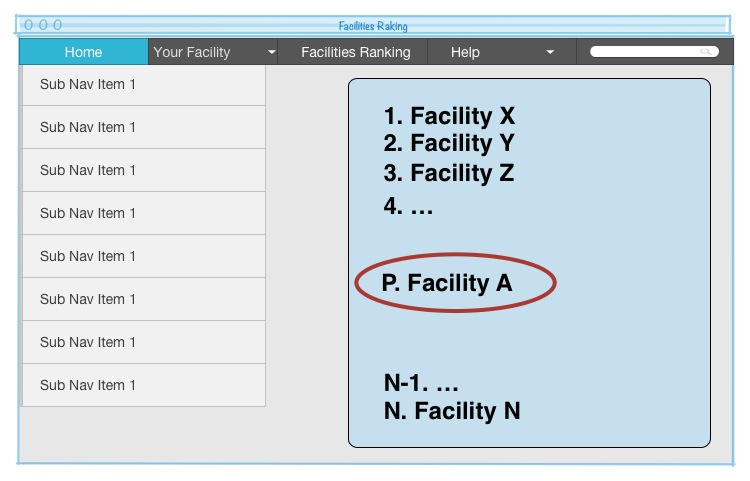
\includegraphics[width=1\textwidth]{images/raking2.jpeg}
  \label{fig:importanceXfrequency}
\end{figure}
\end{frame}
\note[itemize]{
	\item vamos supor que existe uma aplicação que agrega informação de várias organizações e faz um raking entre elas
	\item 
	\item {\bf Scenario 1} Consider an organization that has applied FM and where benchmarking has been applied for some time now. This organization decides to use the application proposed in this document. Through it, verifies that its position is raking well below than expected. Thus, seeing their ranking, they become motivated to improve (as they have a perception of their space for improvement) both globally and at the level of a particular indicator.
	\item ainda há um caminho de melhoria, e a gestão de fm começou a percorrer um caminho de melhoria.
}

\begin{frame}{Motivation Scenario B}
Continuous Improvement Awareness
\begin{figure}
  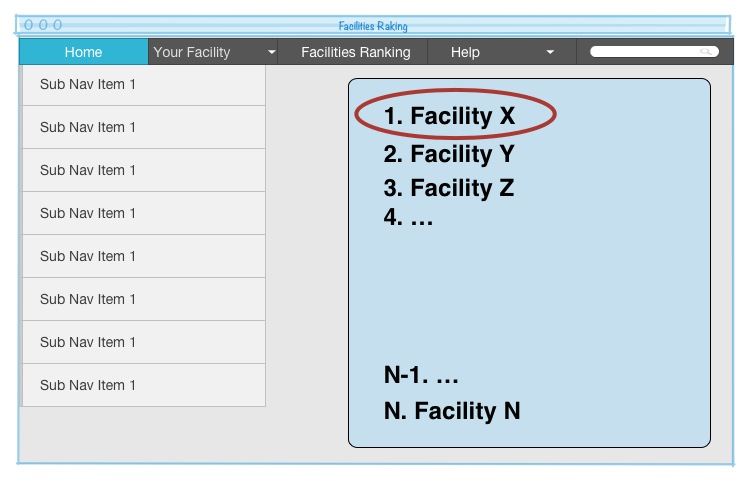
\includegraphics[width=1\textwidth]{images/raking3.jpeg}
  \label{fig:importanceXfrequency}
\end{figure}
\end{frame}
\note[itemize]{
	 \item {\bf Scenario 2} Consider two distinct organizations that are using the cloud application presented in this document. The first organization has been on the raking first place for some time now. However, the second organization took their place in the raking, but the first organization wants to regain its position. Thus, it creates a healthy competition among participants (who do not know the identity of the other), where improvement is still driven dynamically.
	 %\item vai ser despoletada a consciencia nos agentes de gestão de possibilidade de uma conit

}

\begin{frame}{Motivation-Scenario 2}
Continuous Improvement Awareness
\begin{figure}
  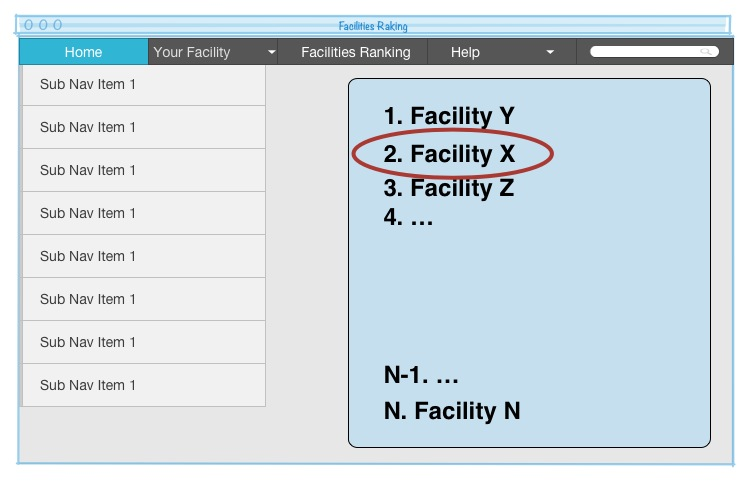
\includegraphics[width=1\textwidth]{images/raking4.jpeg}
  \label{fig:importanceXfrequency}
\end{figure}
\end{frame}
\note[itemize]{
	 \item {\bf Scenario 2} Consider two distinct organizations that are using the cloud application presented in this document. The first organization has been on the raking first place for some time now. However, the second organization took their place in the raking, but the first organization wants to regain its position. Thus, it creates a healthy competition among participants (who do not know the identity of the other), where improvement is still driven dynamically.
	% \item Entrar em detalhe que é importante ter kpis para comparaçao
	% \item Ha aqui 2 detalhes muito importantes:
	% \item Os kpi para fazer as medições
	% \item O benchmarking para comparação de facilities

		 \item Se uma solução destas existisse, tornaria clara uma consciencialização dos gestores de facilities para uma melhoria sustentada das suas facilities. A partilha de informação de benchmarking é uma ferramenta que permite aumentar a consciencia da necessidade de melhoria.
	 \item Nesta área de gestão, já foram estudados processos de melhoria continua, são baseados em indicadores de performance, em particular no FM, são conhecidos por Key performance indicators.
}

\begin{frame}{Key Performance Indicators}
	Through the FM software is possible to extract measures which are used to calculate Key Performance Indicators (KPIs)\\ 
	\vspace{0.5cm}
	KPIs give important insight into functioning of the FM functions\\

	\begin{block}{KPIs Examples}
	\begin{itemize}
		\item {\bf Cleaning Cost per $m^2$:} Total Cleaning Costs/Net Floor Area
		\item {\bf Repairs VS Preventive Maintenance:} (Number of Corrective Maintenance per month/Number of Preventive Maintenance per month)x100
		\item {\bf Quality of Cleaning:} Obtained Through Audits or Questionnaires
	\end{itemize}
	\end{block}

\end{frame}
\note[itemize]{
\item Através do software de FM falado anteriormente é possível retirar medições e indicadores que podem ser utilizados para calcular Key Performance Indicators (KPIs), que por sua vez dão informação importante sobre o funcionamento das funções FM.
\item No FM há um conjunto de indicadores mais ou menos comuns, e que são conhecidos. Por exemplo, Custo de limpeza por $m^2$, Ratio entre o Numero de Reparações sobre Numero de intervenções preventivas, e qualidade da limpeza.
\item Estes kpis sao obtidos apartir de um conjunto de metricas base, Mais em detalhe, temos o custo de limpeza por $m^2$ é calculado através do total do custo das limpezas a dividir pela área util.
\item Estas métricas são, entao obtidas através do software de fm referido anteriormente.
}

\begin{frame}{Key Performance Indicators}
	\begin{block}{KPIs must be SMART}	
		\begin{itemize}
			\item {\bf S}pecific: well defined and clearly understood
			\item {\bf M}easurable: theres a well defined process that enables the KPI tracking
			\item {\bf A}greed: all stakeholders have to agree with it
			\item {\bf R}ealistic: that can be measured at a reasonable cost
			\item {\bf T}ime driven: if corresponds of a time interval
		\end{itemize}
	\end{block}
\end{frame}
\note[itemize]{
\item KOs KPIs para serem uteis, têm de obedecer a um conjunto de principios, conhecidos por SMART:
\begin{itemize}
		\item Specific: bem definidos e claramente compreendidos
		\item Measurable: o processo bem definido que permite seguir o indicador
		\item Agreed: todos os stakeholders concordam com eles
		\item Realistic: passíveis de serem medidos a um custo razoável
		\item Time driven: devem  corresponder a um determinado intervalo de tempo/tm um intervalo de tempo/pode ser medido no tempo
\end{itemize}
}

\begin{frame}{Key Performance Indicators}
	\begin{block}{KPIs for FM are not always SMART}	
		\begin{itemize}
			\item They are not specific
			\vspace{0.5cm}
			\item They are not a standard measure method
		\end{itemize}
	\end{block}
	\begin{block}{And more...}	
		\begin{itemize}
			\vspace{0.5cm}
			\item There are not even an agreed set of KPIs for FM
		\end{itemize}
	\end{block}
\end{frame}
\note[itemize]{
\item No entanto, verifica-se que os KPIs em FM nem sempre são SMART:
\
\item muitas vezes a sua definição é difusa 
\item
\item nao sao especificos: porque o mesmo aparece com varios nomes (tem muitas variações) - a sua definição é difusa
\item
\item Existem percepções variáveis relativamente à forma como devem ser medidos
\item
\item Mas, como se isto não bastasse, nem sequer há concordância a qual é o conjunto de kpis que é de facto relevante para o FM.
%não existe um conjunto de KPIs standardizados, de forma a que todas as organizações usem os mesmos
}

\begin{frame}{Benchmarking}
	\begin{block}{Benchmarking in Management}
	\begin{itemize}
		\item Organizations have to perform better than their competitors
	\end{itemize}
	\begin{itemize}
		\item Organizations have to operate at the lower costs
	\end{itemize}
	\begin{itemize}		
		\item Benchmarking enables to compare performance aspects 
	\end{itemize}
	\end{block}
	\begin{block}{Benchmarking in Facilities Management}
	\begin{itemize}		
		\item Benchmarking can compare distinct organizations or a facility with itself at different time lines
	\end{itemize}
	\begin{itemize}		
		\item We have to measure the same things
	\end{itemize}
	\end{block}
\end{frame}
\note[itemize]{
\item A motivação para o Benchmarking do ponto de vista de gestão, é que as organizações querem ter um desempenho melhor do que a sua concorrência, em particular o objectivo é fazer melhor, mais depressa, e com custos mais baixos.

\item Relativamente ao FM, 

\item É importante conseguir comparar as organizações e isto é possível através de KPIs e benchmarking

\item Benchmarking permite comparar aspectos de performance como: {\bf Operating costs, Maintenance and Cleaning activities, Space utilization, Energy consumption or Administrative costs}

\item O benchmarking é possível entre organizações, mas também como forma de comparar a mesma organização em diferentes pontos de uma linha temporal, tomando-se conhecimento da evolução da mesma
\item Tem de se fazer benchmarking de forma acordada por todos. As organizações têm de estar a comparar os mesmos indicadores, não existem standards que o permita.

}

\begin{frame}{Benchmarking}
	\begin{block}{Fundamental steps for benchmarking}	
		\begin{itemize}
			\item {\bf Knowing operation} to evaluate internal operation strengths and weaknesses
		\end{itemize}
		\begin{itemize}
			\item {\bf Knowing the industry leaders or competitors} to know the strengths and weaknesses of the competition
		\end{itemize}
		\begin{itemize}
			\item {\bf Incorporating the best} to emulate the strengths of the leaders in competition
		\end{itemize}
		\begin{itemize}	
			\item {\bf Gaining superiority} to go beyond the best practices installed and be the best of the best
		\end{itemize}
	\end{block}
\end{frame}
\note[itemize]{
\item Passos fundamentais para o benchmarking:
\item
\item Conhecer a Operação: para avaliar pontos fortes e fracos da operação interna
\item
\item Conhecer a Concorrência e lideres da industria e os seus pontos fortes e fracos
\item
\item Incorporar o melhor de cada um para fazer frente e competir com os rivais
\item
\item Tentar ser o melhor de todos
}





\section{Problem Statement}
\begin{frame}{Problem Statement}
\fontsize{20}{10}\selectfont
There is not an agreed set of KPIs or a benchmarking process.
\end{frame}
\note[itemize]{
\item There is not an agreement about which KPI should be applicable in each sector
\item
\item Nao se sabe muito bem que kpis se deve utilizar, nao ha um conjunto kpis neste momento que seja aceite por todos
\item
\item Existe uma falta de soluções de FM que permitam integrar informação de diferentes organizações por forma a dar-lhes ganhos
\item
\item As organizações continuam a usar softwares distintos para o seu FM e aglomeração de KPIs

}

\begin{frame}{Methodology}
	\begin{block}{Analysis of Related Work}
	\begin{itemize}
	\item Analysis of existent standards for FM
	\end{itemize}
	\vspace{0.5cm}
	\begin{itemize}
	\item Analysis of scientific literature about selection of KPIs
	\end{itemize}
	\vspace{0.5cm}
	\begin{itemize}
	\item Analysis of existing tools for FM and benchmarking
	\end{itemize}
	\end{block}
\end{frame}
\note[itemize]{
	\item Então como se pode resolver este problema?
	\item
	\item 1) O primeiro passo será fazer um levantamento dos standards existentes
	\item
	\item 2) Uma analise da literatura
	\item
	\item3) Analise de ferramentas de FM e Benchmarking 
}

\begin{frame}{Methodology}
	\begin{block}{Matrix Elaboration}
	\begin{itemize}
	\item Elaboration of a normalized and prioritized KPI matrix
	\end{itemize}
	\end{block}
	\vspace{0.5cm}
	\begin{block}{Matrix Validation}
	\begin{itemize}
	\item Cross-over of KPI matrix with experts opinion
	\end{itemize}
	\vspace{0.5cm}
	\begin{itemize}
	\item Evaluation of conclusions through a cloud application
	\end{itemize}
	\end{block}
\end{frame}
\note[itemize]{ 
	\item4) Para tentar chegar à conclusao de uma matriz de kpis, que sofre uma  normalização dos indicadores (para baterem certo uns com os outros) e 
	\item
	\item5) Prioritização de indicadores, Cruzamento de dados da matriz de KPIs com a opniao de experts na área.
	\item
	\item6) E vamos avaliar isso atraves de uma aplicação cloud que vai permitir aceder aos KPIs de cada edificio, bem como uma comparação entre várias organizações
}

% \begin{frame}{Final Goal}
% 	\begin{itemize}
% 		\item Migration of facilities benchmarking to the cloud
% 		\item Design a solution of a cloud application that would receive all important data from multiple sources and calculate KPIs 
% 		\item Carry out a benchmark comparison between organizations through the proposal solution
% 	\end{itemize}

% \end{frame}
% \note[itemize]{
% \item la
% }


\section{Related Work}
\subsection{SOMs}
\begin{frame}{The GEO SOM}
  \begin{block}{GEO SOM}
    \begin{itemize}
      \item Applies the first law of geography “Everything is related to everything else, but near things are more related than distant things".
      \item  Defining a variable $k$ which is used as a ``geographical tolerance" that forces the winning neuron to be geographically near the input pattern.
      \item selection of the winning neuron is done in two steps. First, geographic neurons inside the tolerance $k$ with the input data as a center are selected. Only after that, comparisons are made with the rest of data present in the input data.
    \end{itemize}
  \end{block}
\end{frame}
\note[itemize]{
      \item Applies the first law of geography “Everything is related to everything else, but near things are more related than distant things".
      \item  Defining a variable $k$ which is used as a ``geographical tolerance" that forces the winning neuron to be geographically near the input pattern.
      \item selection of the winning neuron is done in two steps. First, geographic neurons inside the tolerance $k$ with the input data as a center are selected. Only after that, comparisons are made with the rest of data present in the input data.
}

\begin{frame}{WEBSOM}
  \begin{block}{The WEBSOM self organizing maps}
    \begin{itemize}
      \item  First SOM is called \textit{word category map}  used to find words that have similar meaning.
      \item Second SOM, called \textit{text},  used to cluster the documents.
    \end{itemize}
  \end{block}
\end{frame}
\note[itemize]{
\item by Honkela
\item Websom is used to cluster webpages
\item has two soms
}

\subsection{Twitter}
\begin{frame}{Twitter Natural Language Processing}
  \textbf{ARK Tweet NLP:}
  \begin{itemize}
    \item Built using a maximum entropy Markov model.
    \item Tags words, such as nouns, verbs, etc..
    \item Can tag words, such as abbreviations, emojis and spelling errors. 
  \end{itemize}
  \textbf{Example:}
  \begin{figure}[htpb]
    \centering
    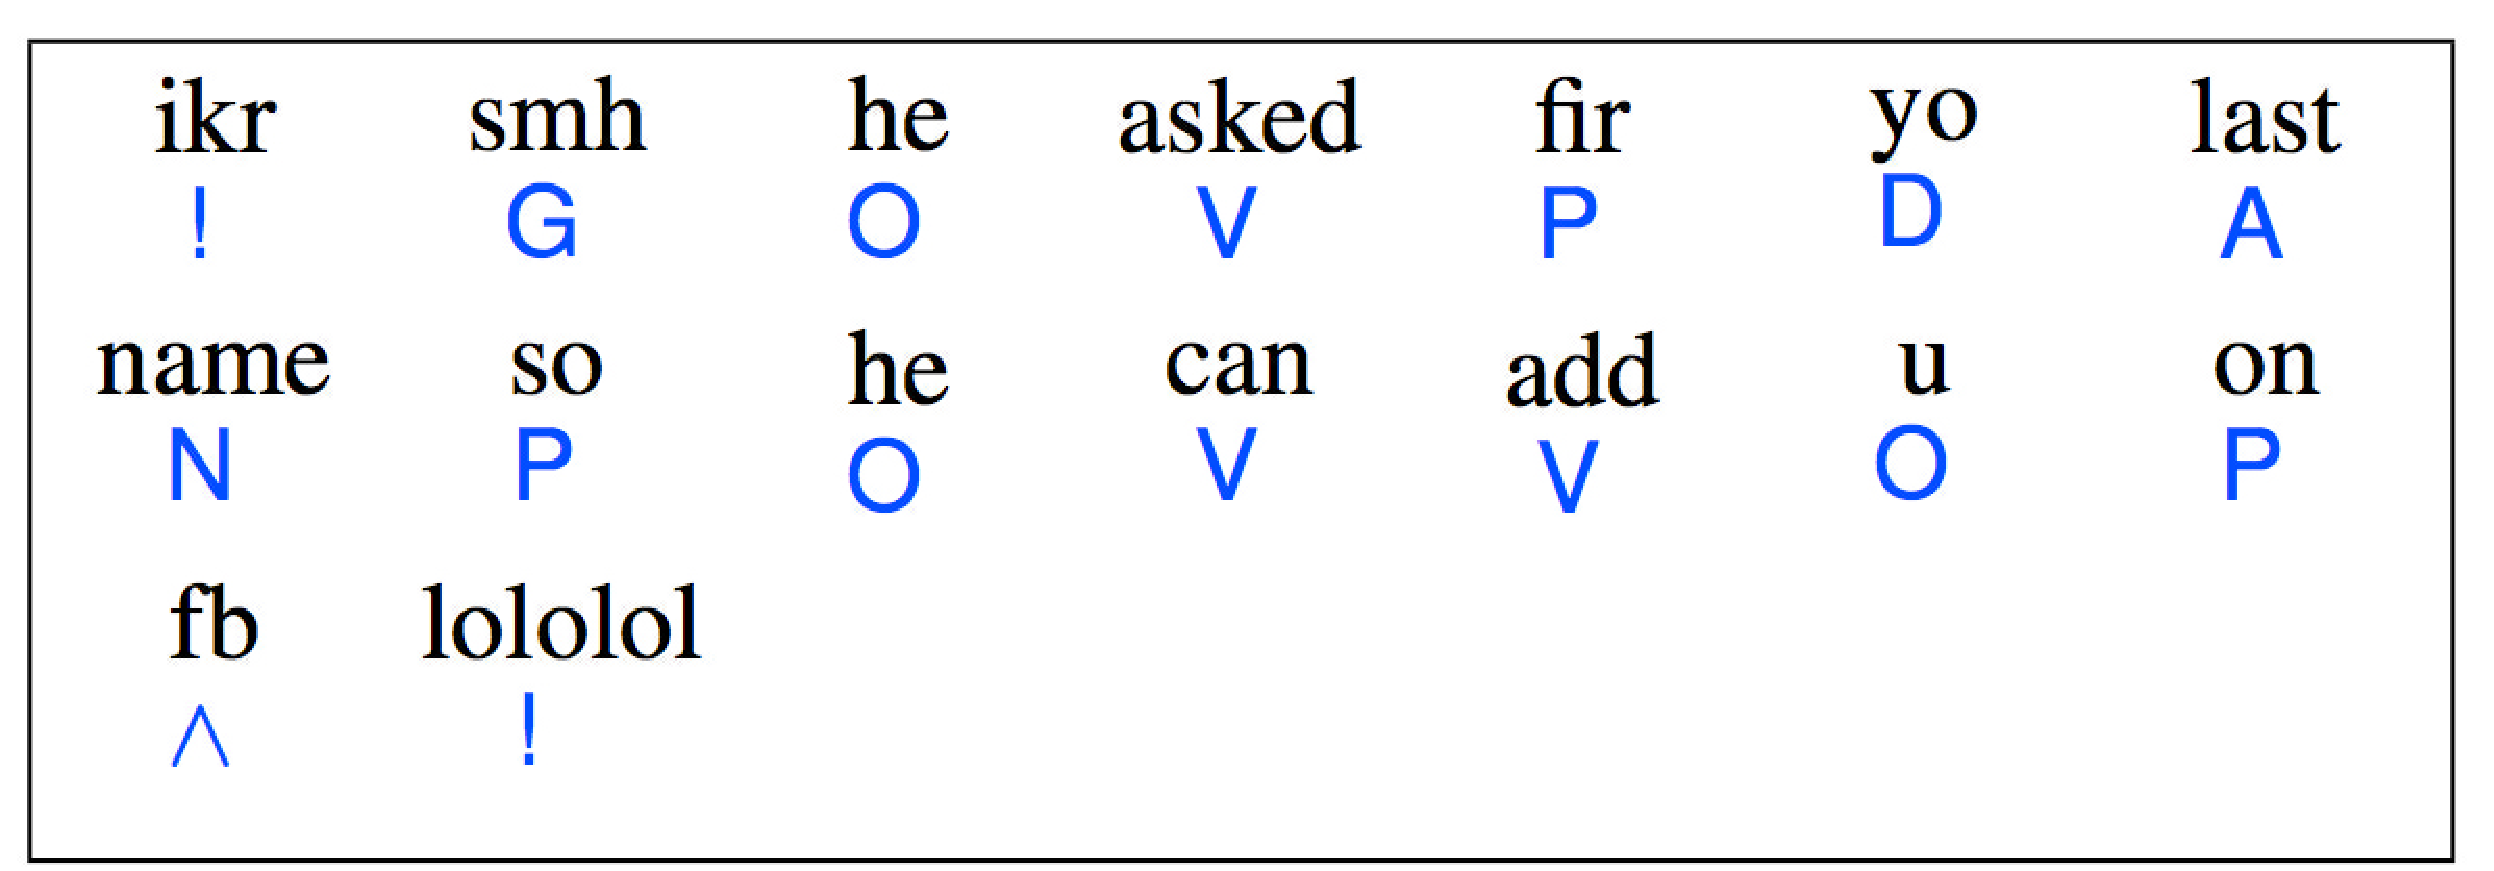
\includegraphics[width=0.6\linewidth]{./images/1_nlp.pdf}
    \label{fig:nlp}
  \end{figure}
\end{frame}
\note[itemize]{
\item Twitter sucks with graphical errors 
\item NLP no twitter antes deste trabalho nao era possivel
  \item Tweet automatically tagged with ARK Tweet NLP. ! stands for interjection, while V stands for verbs and D for determiner.
}

\begin{frame}{Homophily in Social Networks}
  \begin{block}{Miller et al, 2001}
    \begin{itemize}
      \item Similarity breeds connection.
      \item Homophily means \textit{“people like us}.
      \item In diverse societies, race, and race-like ethnicity create the most stark divides.
      \item Sex, age, religion, and education strongly structure our relations with others.
    \end{itemize}
  \end{block}
\end{frame}
\note[itemize]{
\item Not web social, like real social
}

\section{Clustering Tweets with SOMs}
\begin{frame}{VSM Conversion}
\textbf{Problems with direct convertion:}
\begin{itemize}
  \item Words without meaningful content where used.
  \item Similar words where categorized differently.
  \item Symbols near words would render different word.
\end{itemize}
\end{frame}

\begin{frame}{VSM Reduction with String Reducers 1}
  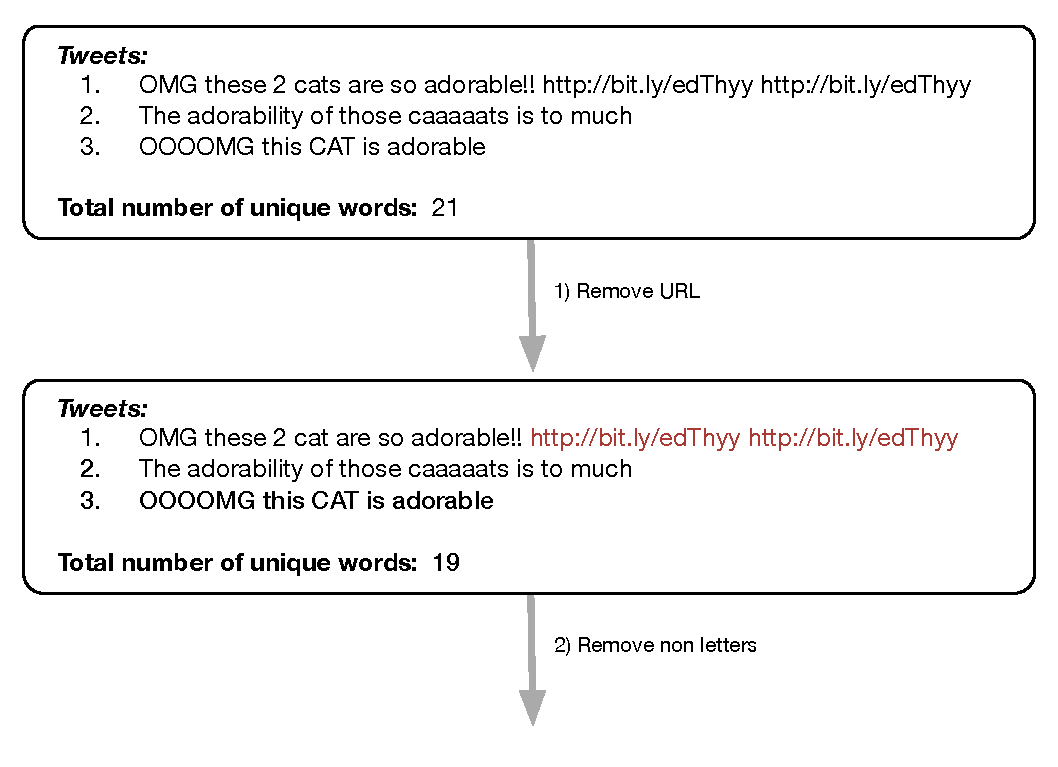
\includegraphics[width=1\textwidth]{images/string_reduction_1.pdf}
\end{frame}

\begin{frame}{VSM Reduction with String Reducers 2}
  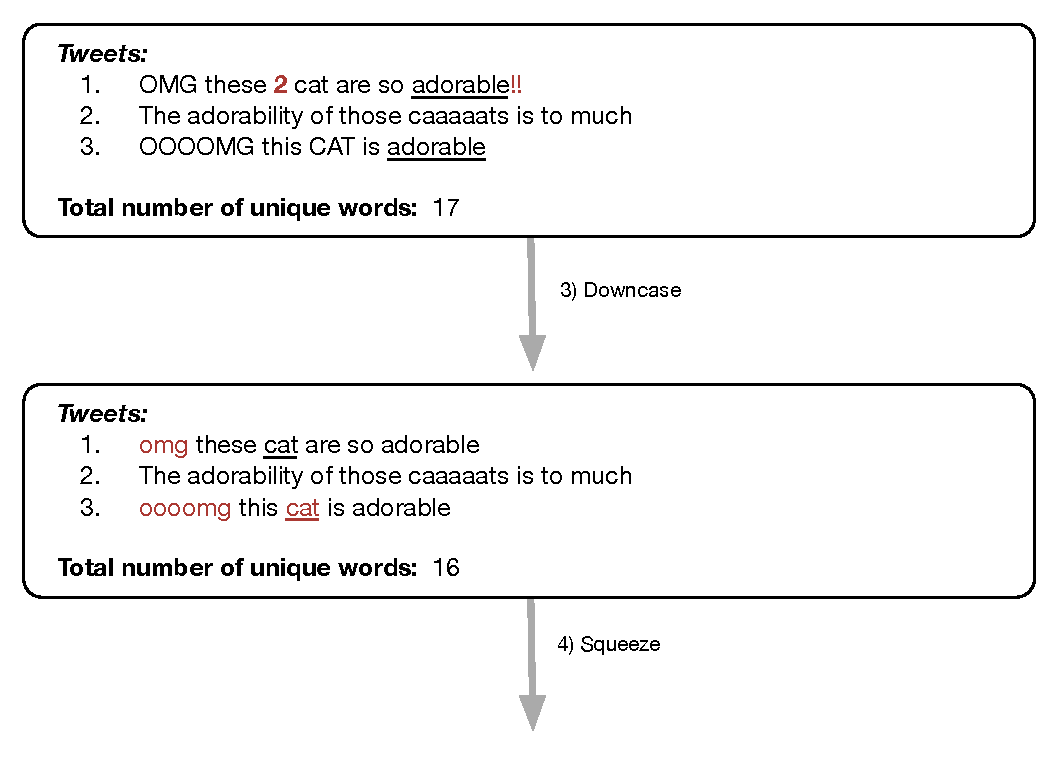
\includegraphics[width=1\textwidth]{images/string_reduction_2.pdf}
\end{frame}

\begin{frame}{VSM Reduction with String Reducers 3}
  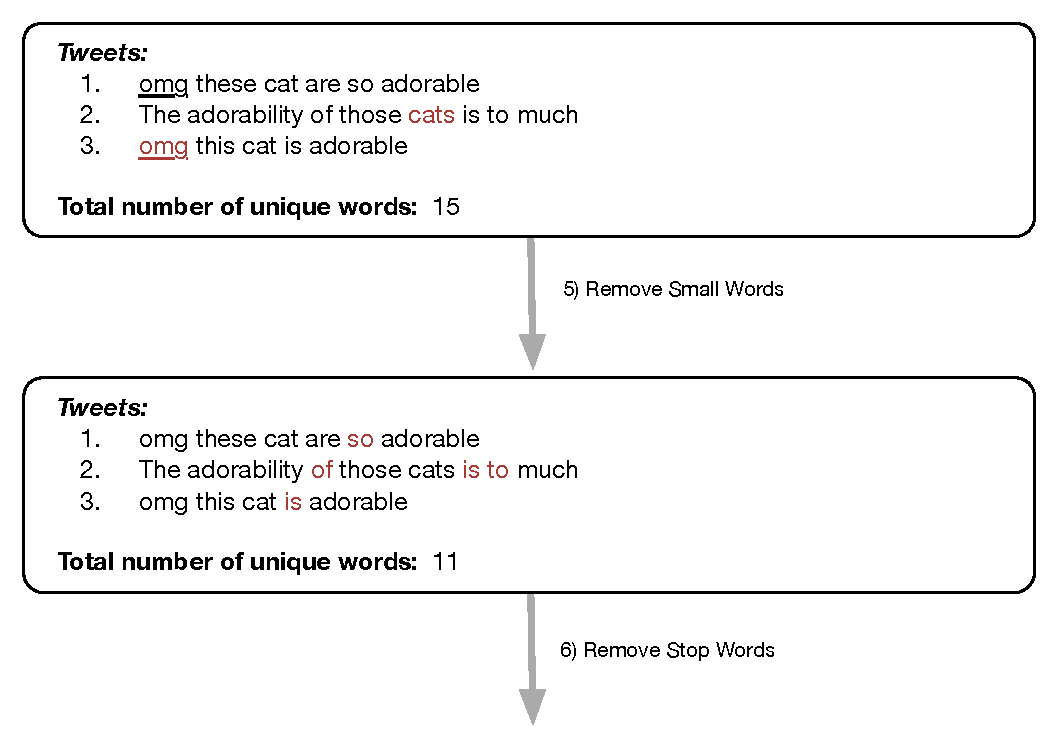
\includegraphics[width=1\textwidth]{images/string_reduction_3.pdf}
\end{frame}

\begin{frame}{VSM Reduction with String Reducers 4}
  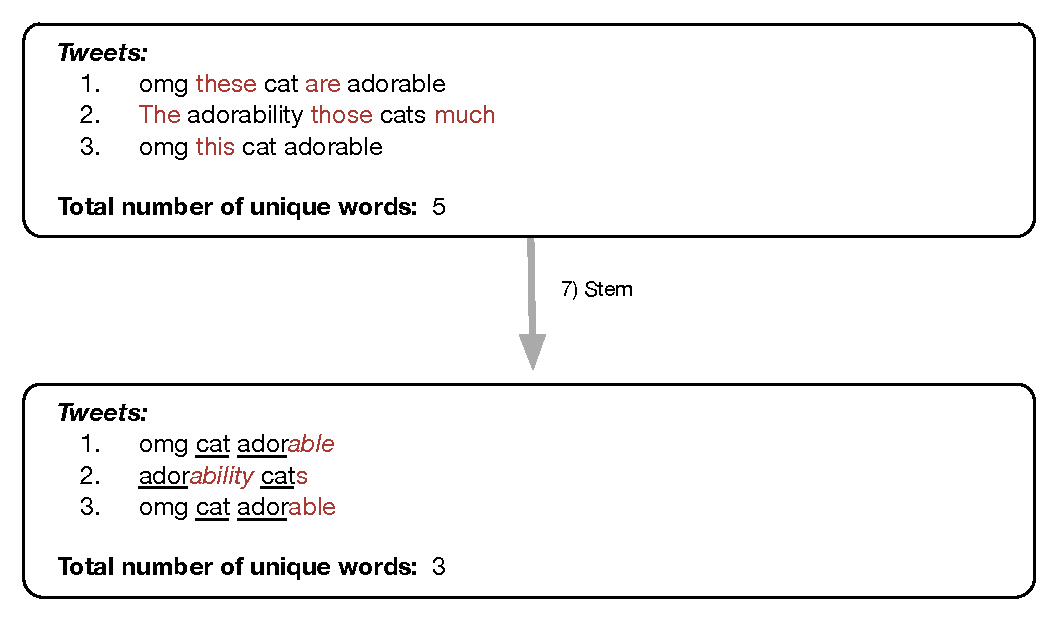
\includegraphics[width=1\textwidth]{images/string_reduction_4.pdf}
\end{frame}

\begin{frame}{VSM Reduction Results}
  \textbf{75\% reduction of total unique words}
  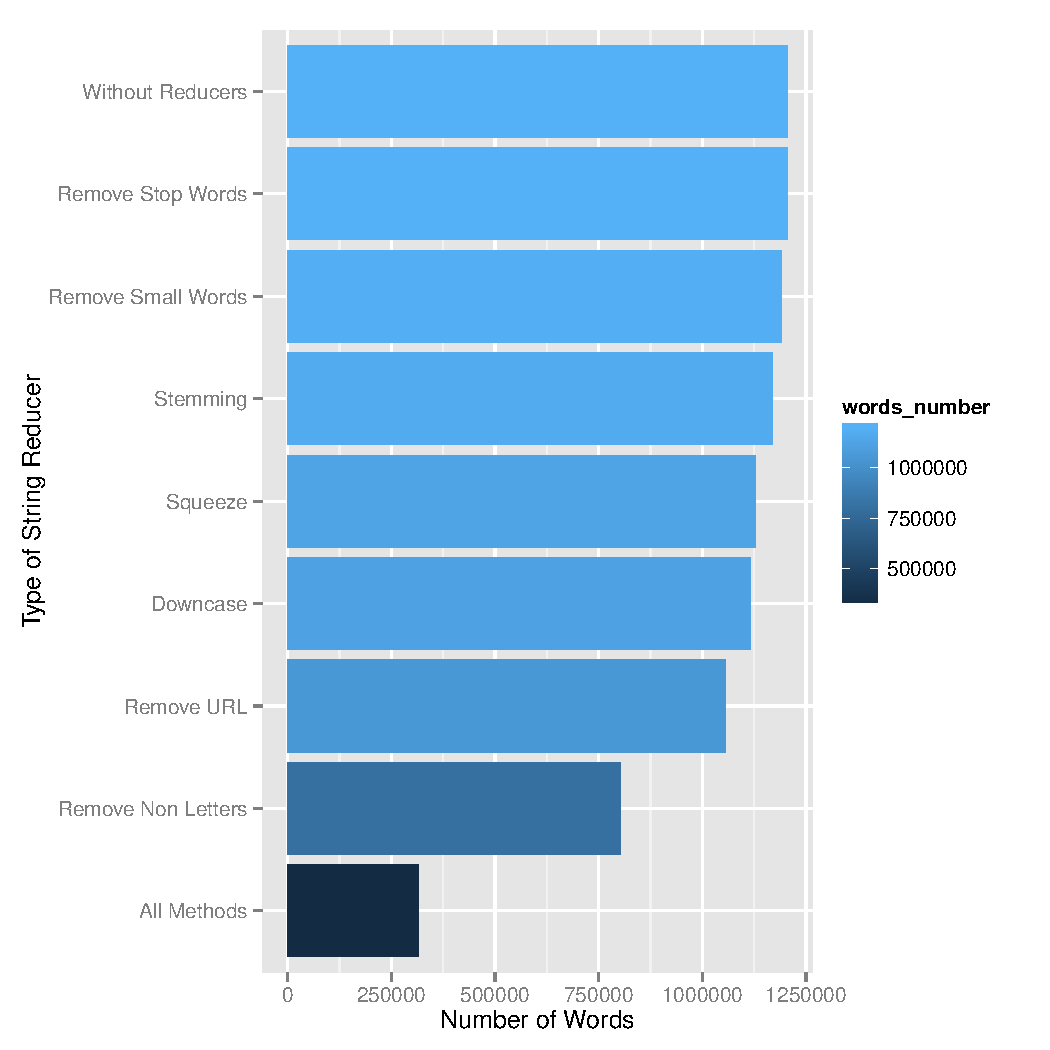
\includegraphics[width=0.65\textwidth]{images/plot_wordcount.pdf}
\end{frame}

\begin{frame}{VSM Reduction with NLP 1}
  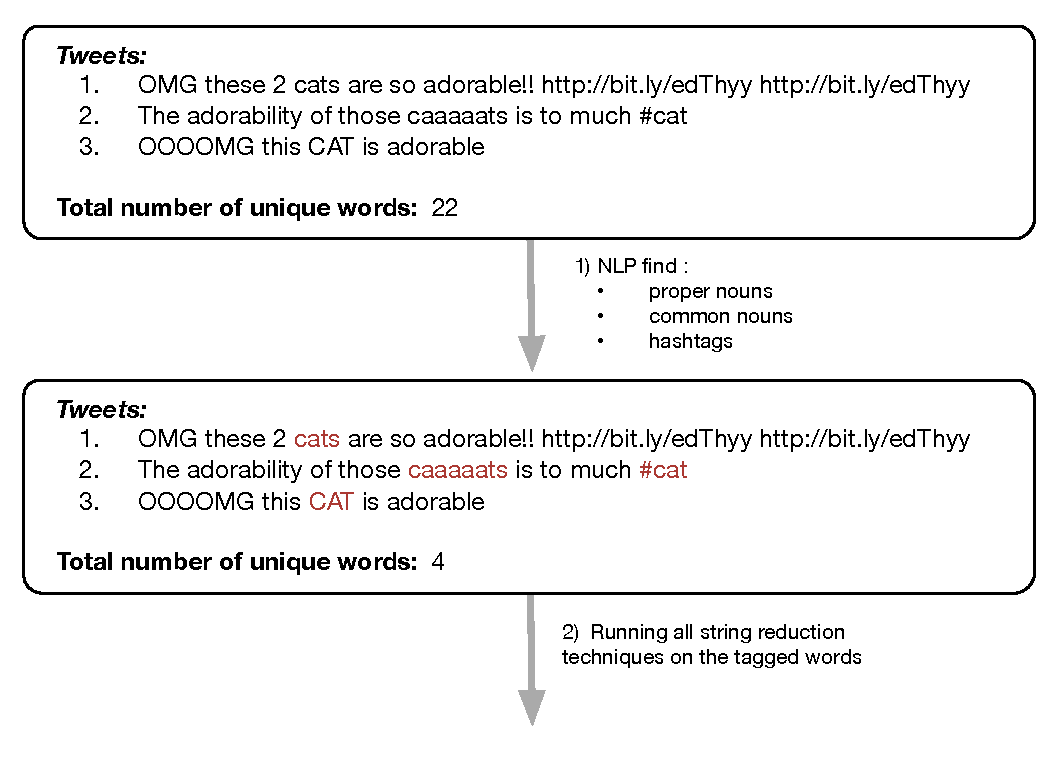
\includegraphics[width=1\textwidth]{images/string_reduction_nlp_1}
\end{frame}

\begin{frame}{VSM Reduction with NLP 2}
  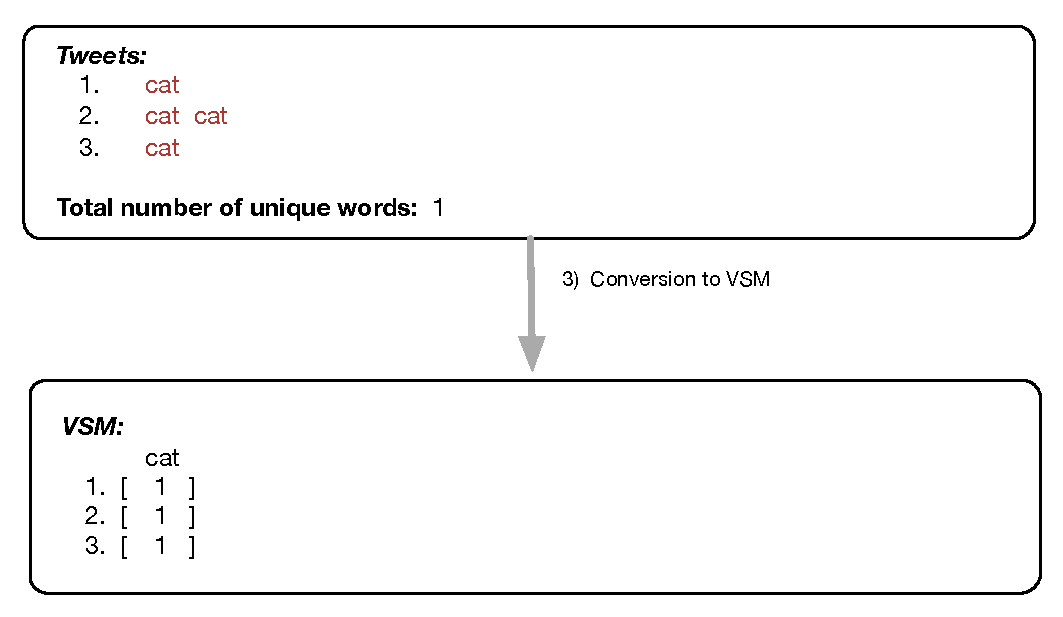
\includegraphics[width=1\textwidth]{images/string_reduction_nlp_2}
\end{frame}

\begin{frame}{VSM Reduction Results}
  \textbf{95\% reduction of total unique words}
  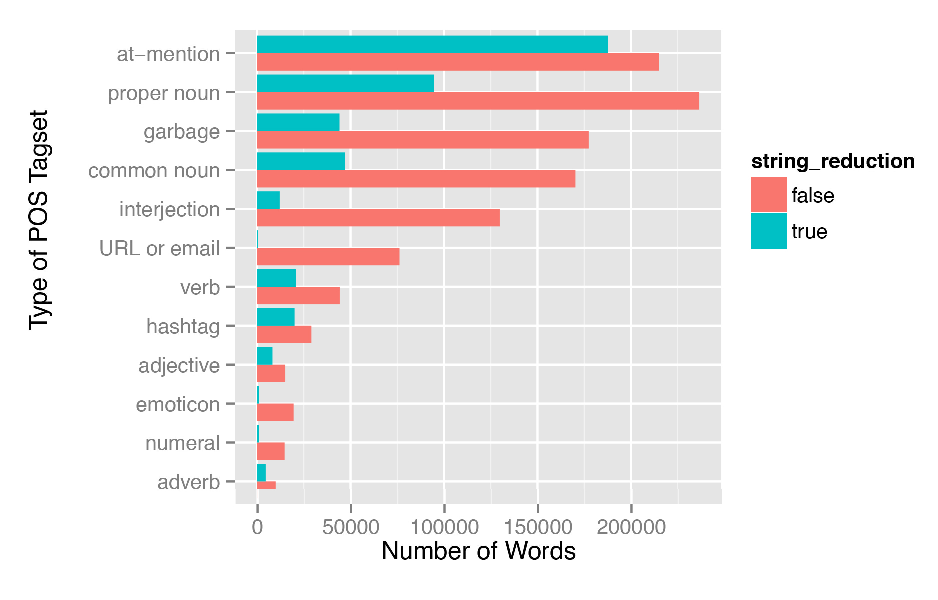
\includegraphics[width=1\textwidth]{images/plot_wordcount_nlp.pdf}
\end{frame}


\section{Enhancing SOM for socially connected data}
\begin{frame}{Homophilic SOM}
  \begin{figure}
    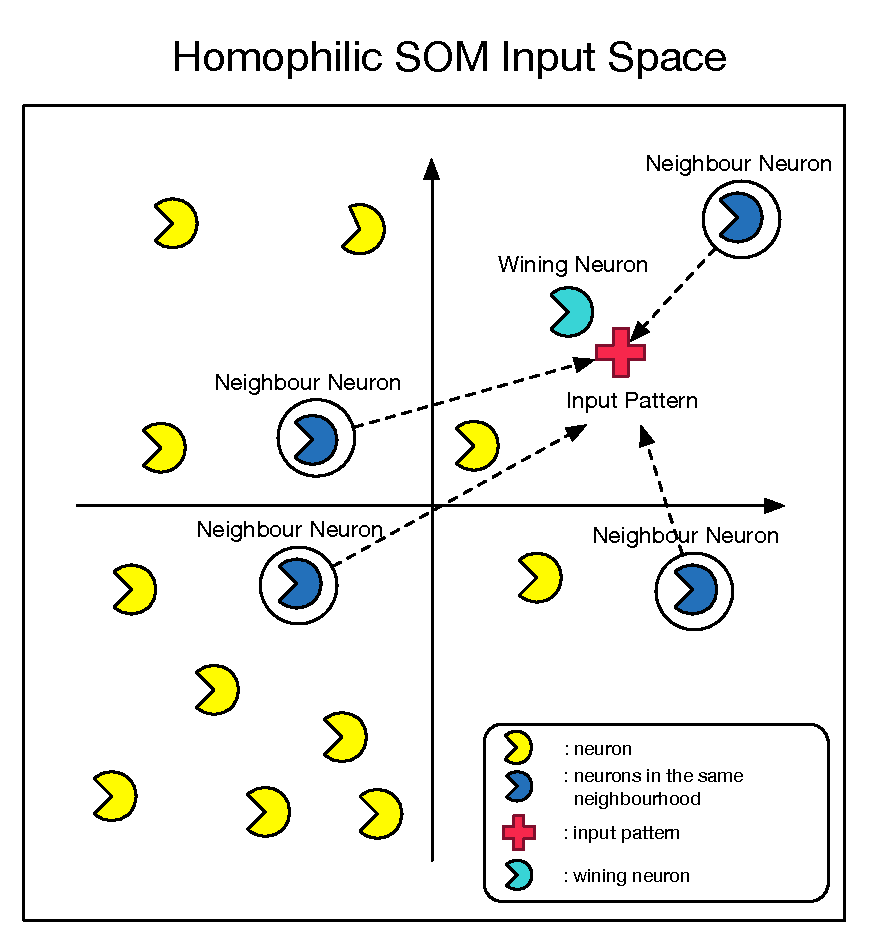
\includegraphics[width=0.5\textwidth]{images/homophilic_input_space.pdf}
  \end{figure}
\end{frame}

\begin{frame}{Homophilic SOM}
  \begin{figure}
    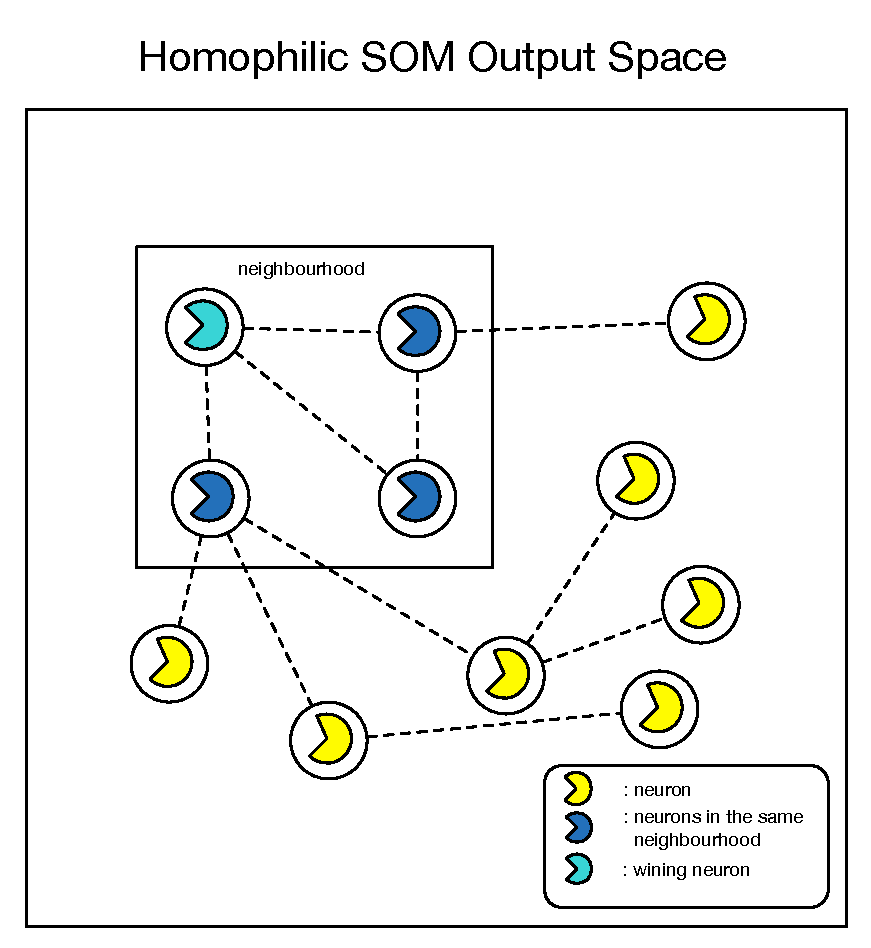
\includegraphics[width=0.5\textwidth]{images/homophilic_outputspace.pdf}
  \end{figure}
\end{frame}

\begin{frame}{SOM Framework}
  \textbf{Why develop another SOM library? }
  \begin{itemize}
    \item Current SOM libraries don't allow the neighborhood function to be defined before training. 
    \item A lot of customizations to the SOM algorithm where made, and each has its own code. 
    \item SOM implementations on higher level languages rely on C. 
    \item Easy to test new SOM approaches.
  \end{itemize}
\end{frame}

\begin{frame}{Testing SOM Framework}
  \textbf{Using the SOM framework to train a SOM to identify different colors:}
  \begin{figure}
    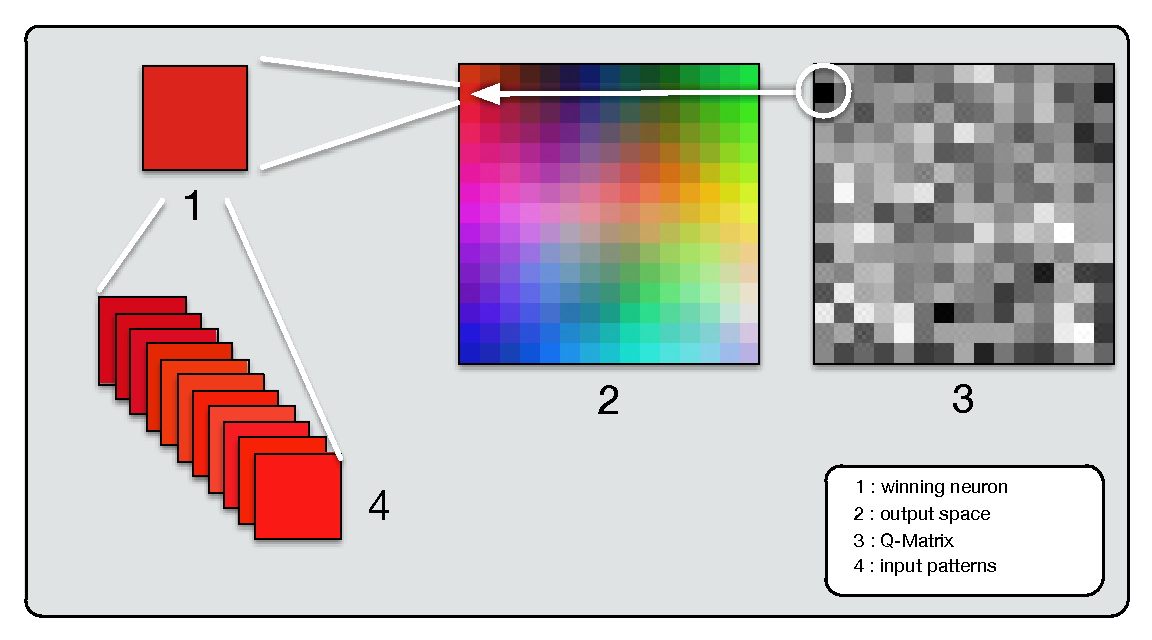
\includegraphics[width=1\textwidth]{images/som_trainned.pdf}
  \end{figure}
\end{frame}

\begin{frame}{Homophilic SOM Implementation}
  \begin{itemize}
    \item On top of the SOM framework.
    \item Changed the Output Space class, which was no longer squared.
    \item Everything keeps working as it was supposed to.
  \end{itemize}
\end{frame}

\begin{frame}{Homophilic SOM Results}
  \begin{itemize}
    \item I think I haven't had a segmentation fault in years
    \item Just bought a banana phone at \#bananamarket
    \item Real Software Engineering by @glv via @confreaks. @daviddias you're going to enjoy this (it is not about ruby)
    \item R vrs SAS, interesting debate: 
    \item I'm finding @duckduckgo to be pretty more reliable than google when searching for code. Gonna try it as my default se.
    \item Mind blowing results! Taking Commercial 3DP into the Nano Dimension - \#3DPrinting | @scoopit 
  \end{itemize}
\end{frame}


%====================================================================================	
\section{Conclusions}

\begin{frame}{Conclusions}
	%\begin{block}{Nowadays}
	\begin{itemize}
		\item There is no commonly agreed set of metrics to compare facilities
	\end{itemize}
	%\end{block}

	%\begin{block}{This work}
	\begin{itemize}
		\item Analysis of existents standards
	\end{itemize}
	\begin{itemize}
		\item Proposal of a set of KPIs
	\end{itemize}
	\begin{itemize}
		\item Validation through the cloud proposal solution
	\end{itemize}
	% \begin{itemize}
	% 	\item Quantifying real property performance will be easier
	% 	\item Organizations will have a better way to evaluate its own FM metrics
	% 	\item The comparison of metrics between enterprises and facilities will be possbile.
	% \end{itemize}
	%\end{block}
\end{frame}
\note[itemize]{
\item Não existe ainda uma forma acordada de fazer benchmarking nem um conjunto de métricas de comparação de facilities.
\item
\item Neste trabalho fizemos uma analise aos diferentes standards existentes, literatura cientifica e softwares de FM
\item
\item Propusemos uma lista de KPIs a serem utilizados por todas as organizações
\item
\item E uma forma de os validar através de uma solução de software cloud
% \item nowadays achieving an affective portfolio of oprations management is still a challenge
% \item
% \item there is no commonly agreed set of metric to compare facilities
% \item
% \item este trab faz uma analise das diferentes standards q existem e faz uma proposta de indicadores a serem utilizados para o benchmarking entre facilities
% \item
% \item vai fazer uma validaçao com uma aplicaçao cloud que queremos que seja standard

}

\begin{frame}
\begin{center}
\huge Thank you!
\vspace{0.5cm}

\Large Questions?
\end{center}
\end{frame}
\note[itemize]{
\item
}
\end{document}


